\section{Citizens Broadband Radio Service (CBRS)}
민간 광대역 무선서비스(Citizens Broadband Radio Service, CBRS)는 미국이 군사·위성 등 공공용으로 사용하던 3.5GHz 대역 150MHz폭(3,550~3,700MHz)에 혁신 주파수 공유 기술을 접목하여 상업용으로 개방하는 주파수 활용 서비스다. \\
%Textwidth가 조판되는 가로영역의 길이의 변수라 앞에 width의 계수로 그림의 크기 조절 가능
\vspace{-4mm}  
    \begin{figure}[!h]\centering
		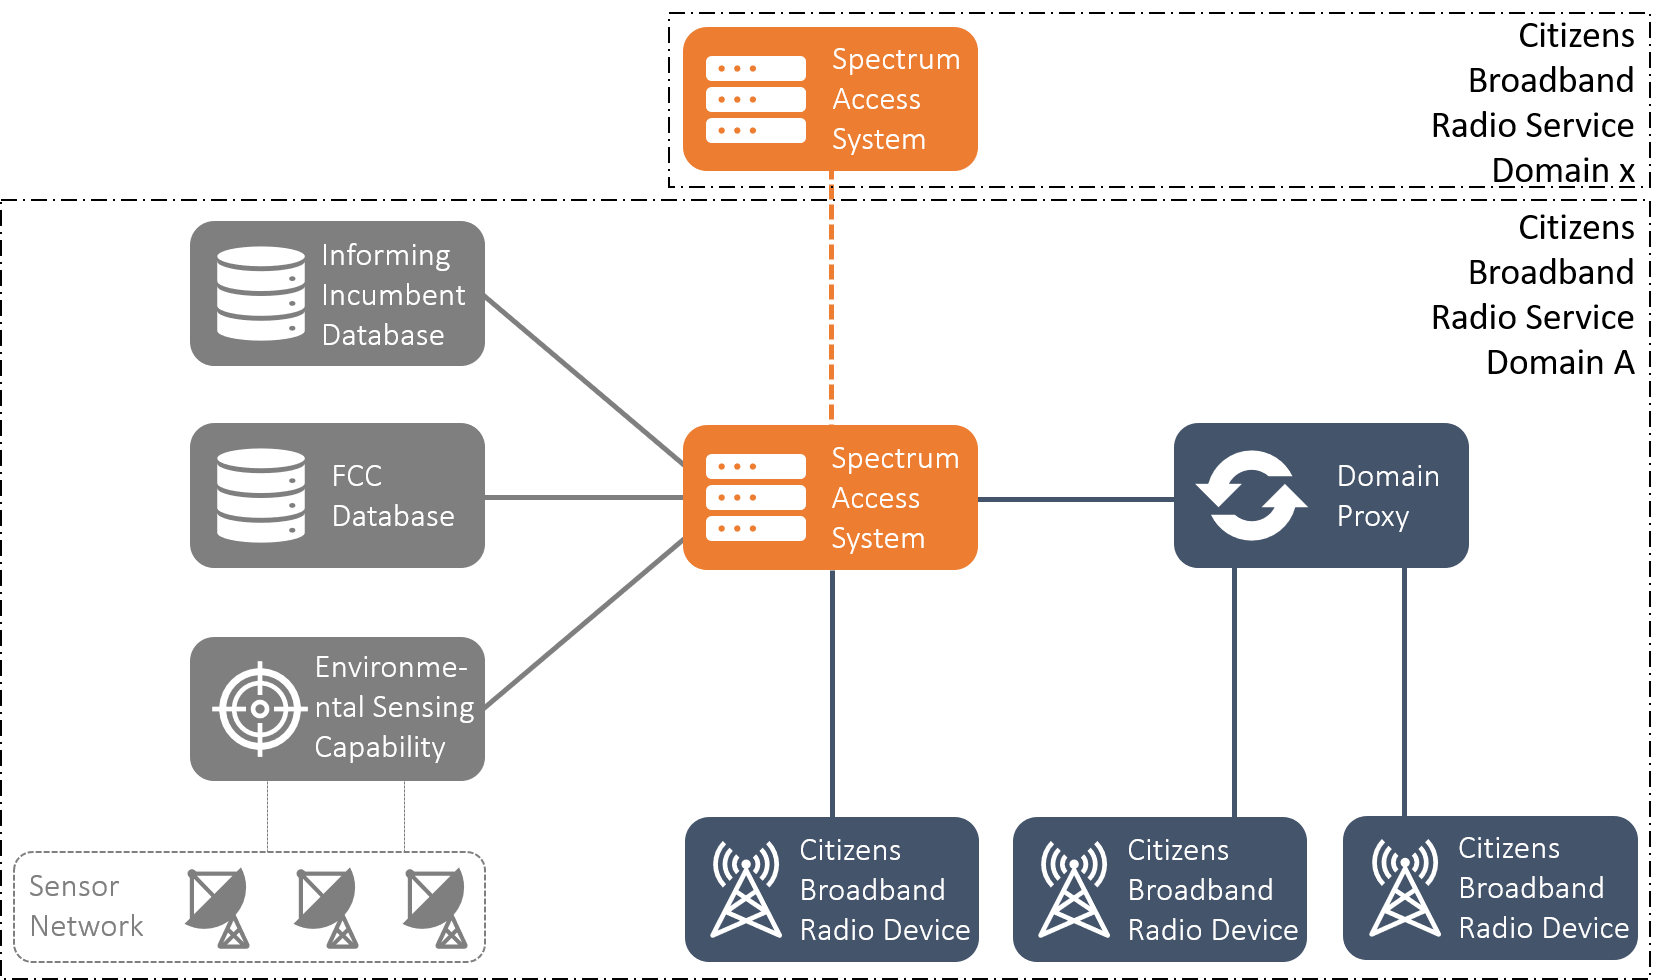
\includegraphics[width=.75\textwidth]{image/week02/1-1.png}
		\caption{\small The Citizens Broadband Radio Service (CBRS) Control Architecturer}
		\vspace{-10pt}
    \end{figure}

CBRS는 총 150MHz의 대역을 우선 순위에 따라 세가지 이용자 계층으로 구분하여 할당한다. 미국 군사·위성과 같은 기존 사용자가 가장 높은 접속 권한을 갖는다. 다음 우선 순위는 미연방통신위원회(FCC)로부터 우선접속권한(Priority Access License, PAL)을 획득하여 기존 사용자가 사용하지 않는 주파수의 일부를 배타적으로 활용하는 사용자이다. 마지막은 일반허가접속(General Authorized Access, GAA)으로, 앞의 2가지 유형의 사용자가 활용하고 남은 대역대를 와이파이와 같은 비면허 대역으로 자유롭게 활용하는 사용자이다. \\
\vspace{-4mm}  
    \begin{figure}[!h]\centering
		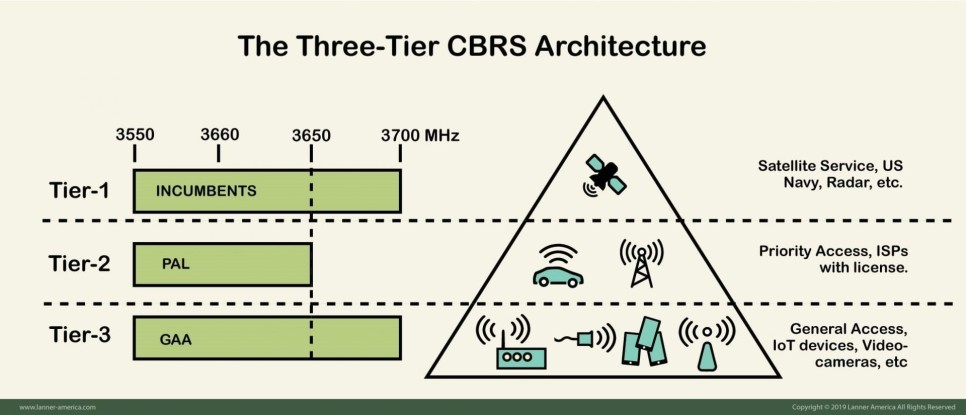
\includegraphics[width=.75\textwidth]{image/week02/1-2.png}
		\caption{\small The Tree Tier CBRS Architecture}
		\vspace{-10pt}
    \end{figure}

이러한 3가지 계층은 동시에 CBRS 주파수를 공유하기 때문에 FCC가 주파수접속시스템(Spectrum Access System, SAS)를 이용하여 모든 주파수 현황을 관리한다. PAL은 기존 사용자를, GAA는 기존 사용자와 PAL을 간섭하지 못하도록, 미사용 채널을 지능형 기술로 실시간 파악하고 이용자들에게 할당한다.

통신사들은 CBRS를 4G LTE 및 5G 네트워크의 적용 범위와 용량을 확장하는데 활용하기를 기대한다. 일반 기업들은 이 주파수 대역을 활용해 자체 4G 및 5G 네트워크를 구축할 수 있다.

기업들은 CBRS를 WiFi 대체 또는 보완 서비스로 활용하거나 IoT 연결, 스마트팩토리 등 공장자동화시스템, 보안 시스템, 사내 사설네트워크 구축 등에 활용할 수 있다.

CBRS는 WiFi와 달리 LTE를 기반으로 하기 때문에 속도가 빠르고 안정적인 연결을 가능하게 한다. 일반적인 WiFi와 비교할때 실내에서 4배, 실외에서 10배의 적용범위를 제공한다. 또한, LTE를 기반으로 하여 보안이 뛰어나며, 일반 사용자(GAA)는 무료로 사용 가능하다는 장점이 있다.
        